\documentclass{standalone}
\usepackage{tikz}

\begin{document}

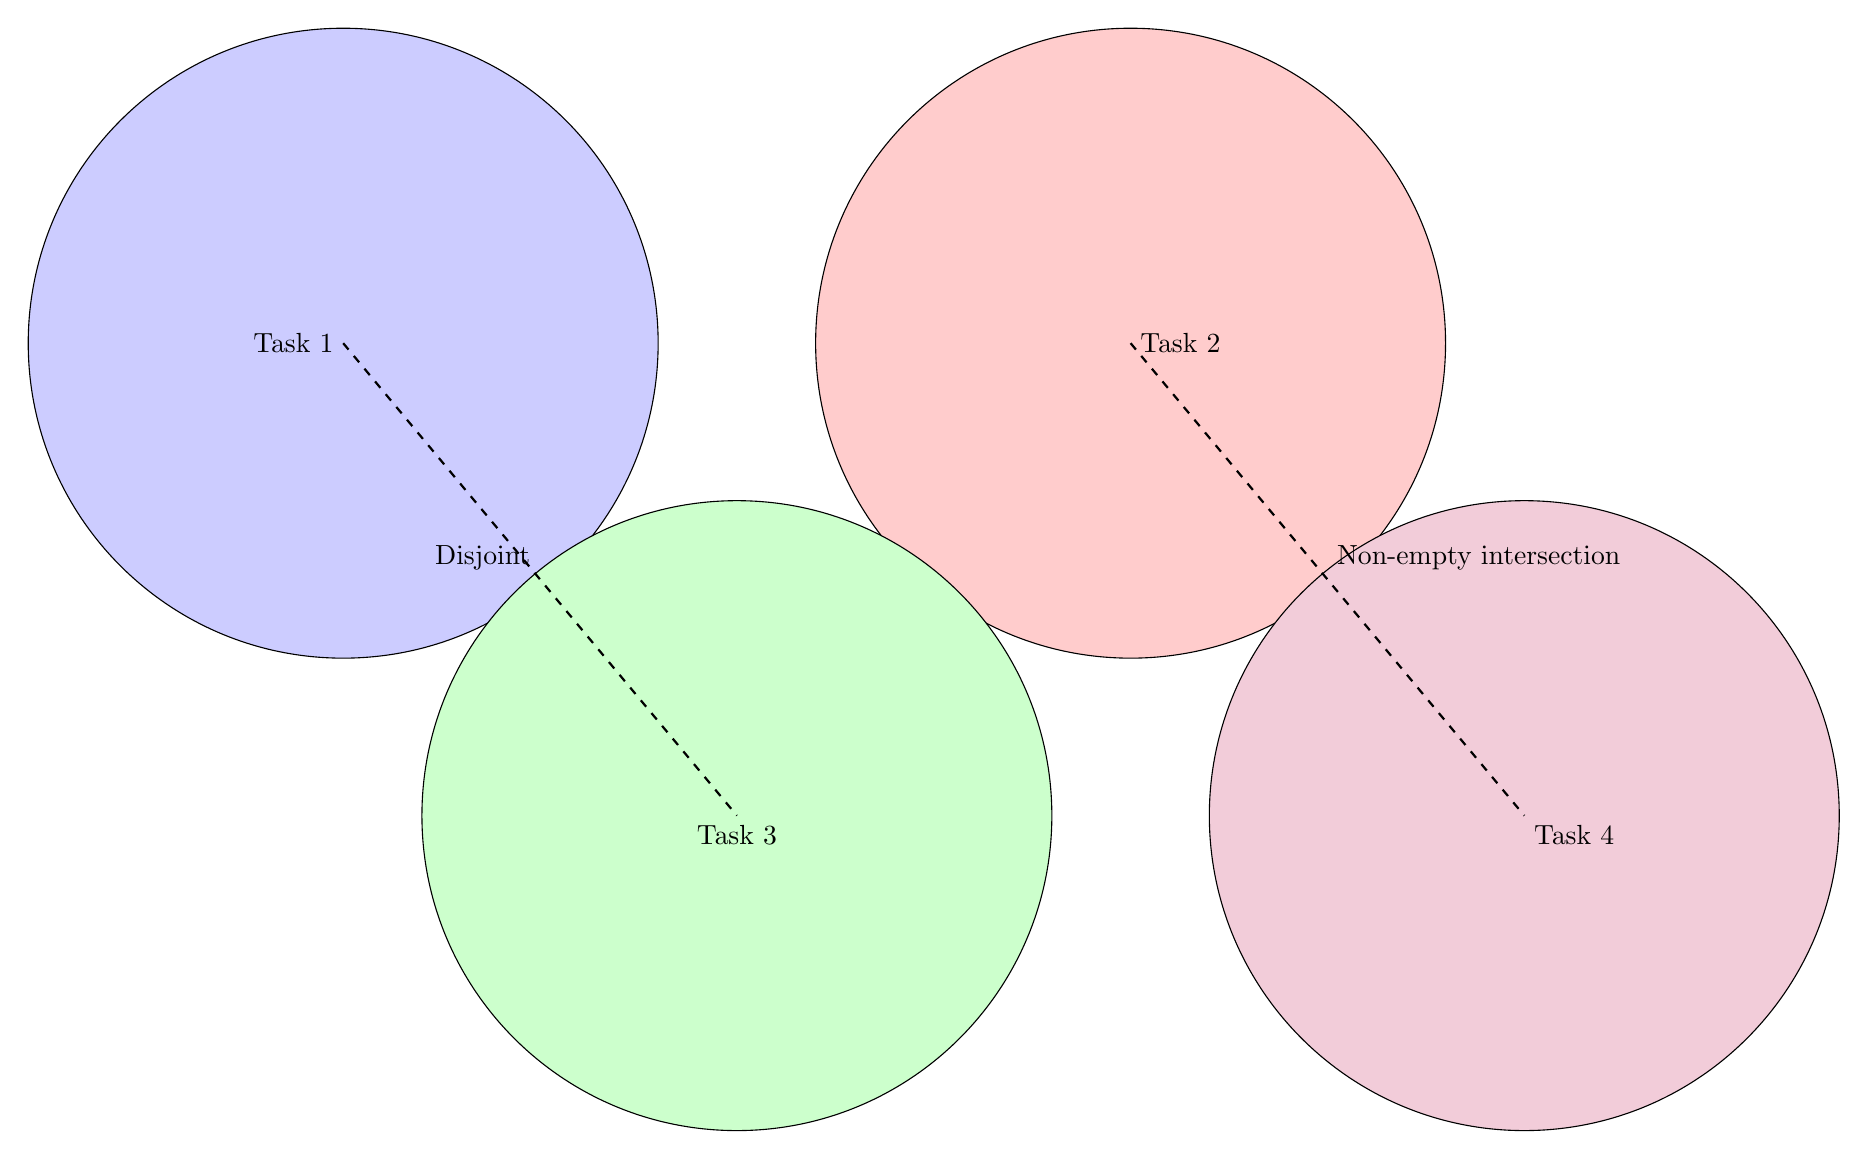
\begin{tikzpicture}[scale=2]

% Draw circles for S_1, S_2, S_3, S_4
\draw[fill=blue!20] (0,0) circle (2cm) node[left] {Task 1};
\draw[fill=red!20] (5,0) circle (2cm) node[right] {Task 2};
\draw[fill=green!20] (2.5,-3) circle (2cm) node[below] {Task 3};
\draw[fill=purple!20] (7.5,-3) circle (2cm) node[below right] {Task 4};

% Draw lines connecting corresponding points to show intersections
\draw[dashed, thick] (0,0) -- (2.5,-3);
\draw[dashed, thick] (5,0) -- (7.5,-3);

% Label intersections
\node at (1.25,-1.5) [above left] {Disjoint};
\node at (6.25,-1.5) [above right] {Non-empty intersection};

\end{tikzpicture}

\end{document}